\chapter{System design}

In this chapter the previously collected information are used to design the system in detail.
The decision making process for that is documented here as well.

\section{Environment}

The environment of where the systems shall be deployed onto must be known for detailed design decisions, which will be elaborated here.

All Winslow instances are supposed to run inside a Docker container (as requested in \autoref{workflow:desired:docker}).
The host will be a Ubuntu or Debian Linux Servers with some having multiple Nvidia graphics cards.
There will be no graphical user interface available on these servers.

Furthermore, the decision to implement Winslow in Java was made early on.
This has three main reasons, first, the developer is experience in Java development, the server side web framework used is a Java library (see \autoref{design:springboot}) and the company this implementation is for has a focus on Java development, which means if the system is successfully, maintained and possibly extended by another developer, it is highly probable that this developer has knowledge in Java development as well.
 \todo{.cleanup}

%\todo{env: shall be executed on ubuntu/debian linux servers, Docker}

\section{Storage Technology}

Storing and accessing data is one of the main concerns for Winslow.
In almost all use cases, there will be multiple Winslow instances that need to access the storage.
Because of that, it must be accessible from remote and from multiple Winslow instances simultaneously.
For that, the following technologies are reviewed: NFS or SMB/CIFS (\autoref{analysis:storage:organisation}),  GlusterFS (\autoref{glusterfs}), SeaweedFS (\autoref{seaweedfs}), OpenIO (\autoref{openio}), dCache (\autoref{dcache}) and HadoopFS (\autoref{hadoopfs}).

The following criteria were used for comparison, with a scoring system with points from 0 to 3, in which 0 means the best solution and 3 the worst - the lower the overall score the better:

\begin{itemize}
\item \textbf{Installation Overhead}:
How hard and extensive is the installation?
Is there a good documentation?
Is the package provided from within the main repository of Ubuntu, or alternatively, does it provide any other form of easy installation?
Scoring 0 for installation through the main repository, 1 for an external repository, 2 for distribution specific archive, 3 for any other installation.

\item \textbf{Dependencies}:
Are further services required for operation? 
How hard are they to setup?
Do they need any additional configuration?
Scoring 0 for no further dependencies, 1 for dependencies but without the need of configuration,  2 for dependencies that require manual configuration, 3 for dependencies that need to be installed manually and require manual configuration.

\item \textbf{Single Point of Failure}:
Is the solution decentralized and is it failure resilient?
Is it site- or rack-aware or provide replication mechanisms to compensate?
Scoring 0 for completely decentralized, 1 for decentralized but with dependency on centralized backend, 2 for mostly centralized but with load balancing approaches, 3 for no single point of failure mitigations.

\item \textbf{Docker integration}:
How easy is it to integrate with Docker?
Scoring 0 for native support, 1 for native but non-trivial support, 2 for support through additional exports facility, 3 for non-trivial solution.

\item \textbf{Failure concerns}:
Are there any noteworthy concerns?
Was an early local test successful and reliable?
Is it a known technology or \enquote{proven in use}?
Who is developing it and what are the support guarantees?
Scoring 0 for commonly used and no concerns, 1 for minor concerns, 2 for major uncertainty, 3 for abandoned technology.
\end{itemize}

In \autoref{comparision:storage} the results are displayed:

\begin{table}[H]
	\begin{tabular}{l|c|c|c|c|c|c|c}
				& NFS S.& SMB/CIFS S.& GlusterFS & SeaweedFs	& dCache 	& HDFS \\
		\hline
		Inst. 	& 0 	& 1 		& 0 		& 2 		& 3			& 1 \\
		Dep. 	& 1 	& 0			& 0 		& 0 		& 3 		& 1 \\
		SPoF 	& 2		& 3			& 0			& 2 		& 0			& 0 \\
		Docker 	& 0 	& 2 		& 2 		& 3 		& 2 		& 3 \\
		Fail.	& 0		& 0			& 1			& 2			& 2			& 0 \\
		\hline
		Score 	& 3		& 6			& 3			& 9			& 10		& 5 \\
	\end{tabular}
	\caption{Comparison of storage technologies}
	\label{comparision:storage}
\end{table}

The worst scoring tool in this comparison is dCache.
The installation overhead, missing documentation and uncertainty on reliable operation is too high for this project (see \autoref{dcache}).

For similar reasons SeaweedFs is placed second worst.
Local tests could not access SeaweedFs reliable when a node failed and there is no trivial support for Docker nor does it provide an NFS export.
Using it from within Docker would require each container to be manipulated so that the first operation is mounting the storage with a custom binary and through a FUSE\footnote{Filesystem in Userspace} mount.
The tool also seems to be developed by a single person which introduces further uncertainty about reliability and support in the future.

HDFS and SMB/CIFS seem to be no terrible choice, but no especially good one either in this use case.

The two best scoring storage solutions are a simple NFS share and GlusterFS.
While GlusterFS provides replication and decentralized access, a NFS share scores with its simplicity.
The idea is to start with a plain NFS share for Winslow which can natively be utilized by Docker as volume mount and to revisit later whether the need for replication and decentralization persists.
Because of the NFS interface export of GlusterFS, Winslow could then easily switch to GlusterFS by accessing the NFS export closest to its' instance.



\section{Execution Management}
\todo{.polish}

As noted in \autoref{analysis:layer_1}, the central business logic is to deciding when and issuing stage executions.
Generally speaking, there are two approaches when executing jobs: local or remote. Both will be discussed next.

In the remote approach, the job is executed on another machine and not on the same which has the responsibility to manage the process.
Continuous Integration (CI) platform Jenkins\cite{jenkins:main} does offer this approach.
The so called slave node (Jenkins) is accessed through a native interface (SSH for Linux servers) to copy resources and to start the job process.
In this scenario, the CI instance requires and stores login credentials for every remote machine to be able to login whenever needed.
The system administrator therefore has to create a new user account on the remote machine, install required programs and prepare the environments.
One big risk for this approach is that in case of any security breach on the central CI instance, the attacker is also able to login on all remote machines.

GitLab\cite{gitlab:main} follows the approach, where the system administrator has to manually install the GitLab Runner on the machine that is then able to connect to GitLab and execute jobs.
This runner is responsible in pulling jobs, execute them locally, monitor and report back the outcome.

Winslow is going to follow the local approach.
On each physical machine that is supposed to execute stages, Winslow needs to be installed and connected to the cluster.
The installation is expected to be easy, as is based on starting prepared Docker images.
An election is selecting the instance which is most fitting for a stage execution (see affinity and aversion in \autoref{election:affinity_and_aversion}).
It is expected that each instance can judge this best on its own, as it knows which resources are available.
Work is therefore distributed to an executor as it is detected.



\section{Event Synchronization and Communication}

\begin{comment}
kafka does what? persist events and provides them in an order(?), cant Winslow do this itself, so that no further dependency is required?

\todo{.}
https://docs.microsoft.com/de-de/azure/architecture/microservices/design/interservice-communication


raw TCP (how to connect, centralized? star? tree?) centralized works towards -> centralized master node
broadcast?
microservice REST
event bus? kafka
messaging queue mqtt
NFS provides filesystem, filesystems are kind of standardized

https://kafka.apache.org/protocol
\todo{.}
\end{comment}


As discovered in \autoref{analysis:layer_2} there is a need for an event synchronization across Winslow instances.
Without proper coordination, race conditions could cause stages to be started multiple times simultaneously, corrupt workspaces, configuration or project files.
While starting too many stage executions are only wasting resources, data corruptions can lead to unrecoverable damage.

There are multiple ways to exchange data between systems that do not share the same process or machine.
The most flexible implementation can be achieved by implementing a custom protocol on a raw TCP socket which allows to exchange blobs (Binary Large Objects) between exactly two nodes.
For a blob or message to reach all nodes, a connection to every other node, a centralized broker, another topology such as a tree structure or broadcast messages would be required.
Because this in itself seemed to be a complex subject, third party alternatives were investigated.

Apache Kafka\cite{kafka} is one such alternative.
It is open source, distributed and is focused on providing system wide ordered data and event stream that can be persisted over a certain time period.
But as every third party service, it introduces a dependency on the project.
Not only in regards to interfacing and driver implementation, but also for maintenance and setup.
Each Winslow Image would require to be shipped with a pre-configured Kafka service and the administrator must ensure that these services can reach each other - in addition to storage solution.

\todo{.rework transition}
It would be rather elegant, if an existing connection - the storage - between all Winslow instances could be reused for this.
This could eliminate the need for this third party dependency.
To do so, a mechanism must be found to give each occurring event a sequence number, that is unique system wide.
A new event would not be allowed to be propagated by an instance before it did not process all previous events.
With this idea in mind, messages that can communication all required coordination information are defined  next.

\begin{comment}

\todo{ACID in fundamentals?}
ACID, which stands for Atomicity, Consistency, Isolation and Durability, describes the needs a database must fulfill so that it does not suffer from side effects or data corruption when executing queries.
A series of changes might not be allowed to be intercepted (atomicity), must see and result in consistent data, is not allowed to interfere with simultaneously executed queries and guarantees that once completed successfully, is in fact persistent and will not be lost (durability).

\todo{filesystem is close}

\todo{DB principles: ACID}

\todo{...}

\todo{requires common a way to exchange messages}

\todo{all messages - called events - are published to all nodes}

\todo{using file system as bus}

\todo{clear and globally same order of events}

\todo{events consist of an id, command, time, duration, subject and issuer}

\todo{events might have a duration}

\todo{unspoken requirement: all nodes share the same clock - or one with very little drift}

\todo{usage as synchronization primitive}
\end{comment}

\subsection{Messages}
\todo{this chapter really needs further polishing}

To coordinate the Winslow instances, messages will be exchanged through the common event bus.
Because of the nature of this global event bus, messages are delivered by broadcasting them to all instances.

Because this is a multi instance system which can suffer partial failure, all multi-part operations have to have a timeout, so that a failure is detectable.
Without this timeout detection, one could not detect the absence of finish signal of a multi-part operation, which could potentially block further operations for forever.
The presence of a timeout will not be mentioned again when listing the messages in detail.

To account for transmission delay and clock offsets an additional time padding is granted.
Because of the non-requirement of real-time scheduling this is generously set to 5 seconds.

A message has the following fields:

\begin{itemize}
	\item \textbf{issuer}: The id of the Winslow instance that wrote the message
	\item \textbf{command}: The state change command (described a bit further below)
	\item \textbf{subject}: What the command is about to change
	\item \textbf{timestamp}: The time of when the message was issued
	\item \textbf{duration}: Optionally a non zero time period of the expected duration
\end{itemize}

With this message structure definition, the following commands can be used:

\begin{itemize}
	\item \textbf{LOCK}: Locking a resource, commonly a project.
	A lock is exclusive to the issuer and can only be granted if there exist no lock for the same subject yet.
	\item \textbf{EXTEND}: Extending an ongoing operation by pushing back its timeout.
	This can be used to signal, that a lock is still required although its timeout is close
	The duration of the original event extended and thus the timeout is pushed back.
	The issuer must be the same as did issue the operation that is referred to.
	\item \textbf{RELEASE}: Releasing a locked resource.
	The issuer must be the same node as the one that issued the \textbf{LOCK} previously.
	\item \textbf{KILL}: Non-gracefully stop an operation or destruction of a lock.
	This signals that an operation shall be stopped or that the lock shall be released immediately.
	This can be used to abort an running stage execution.
	\item \textbf{ELECTION\_START}: Signals that an election for a stage execution started.
	The signal must refer to an project that can make progress.
	\item \textbf{ELECTION\_PARTICIPATE}: Signals that the issuer node is capable of executing the next stage of a project.
	It also includes a scoring for the affinity and aversion (more details in \autoref{election:affinity_and_aversion}).
	This message also includes the election it refers to.
	\item \textbf{ELECTION\_STOP}: Signals that an election has finished.
	The participator with the best affinity and aversion scoring is now allowed execute the next stage of the referred project.
	This is signal is only allowed to be issued by the same node that started the election process.
\end{itemize}

\subsection{Synchronization}

In a file system two files with the same path are now allowed to exist, therefore the sequence number of the event to publish can be used as name for the file in a known directory to write events to.
Watching the directory will then result a stream of ordered events.
To publish an event, a naive implementation would fist check the directory for a file for the sequence number of the new event and create it, if it was not found.
But this has a potential race condition: between checking for the file and creating it, another instance could have created the file as well.
Luckily, the POSIX standard provides a flag when creating files, that will expose this conflict by returning an error if \enquote{Both O\_CREAT and O\_EXCL are set, and the named file already exists}\cite{gnu:open}.
This mechanism is also exposed in Java by calling \javacinline{Files.write(..)}\cite{javadoc:files:write} with \javacinline{StandardOpenOptions.CREATE\_NEW}\cite{javadoc:standard_open_options:create_new}.
The behaviour of publishing an event can therefore be summarized in \autoref{event:synchronized_publish}:

\begin{wrapfigure}{l}{0.37\textwidth}
	\centering
	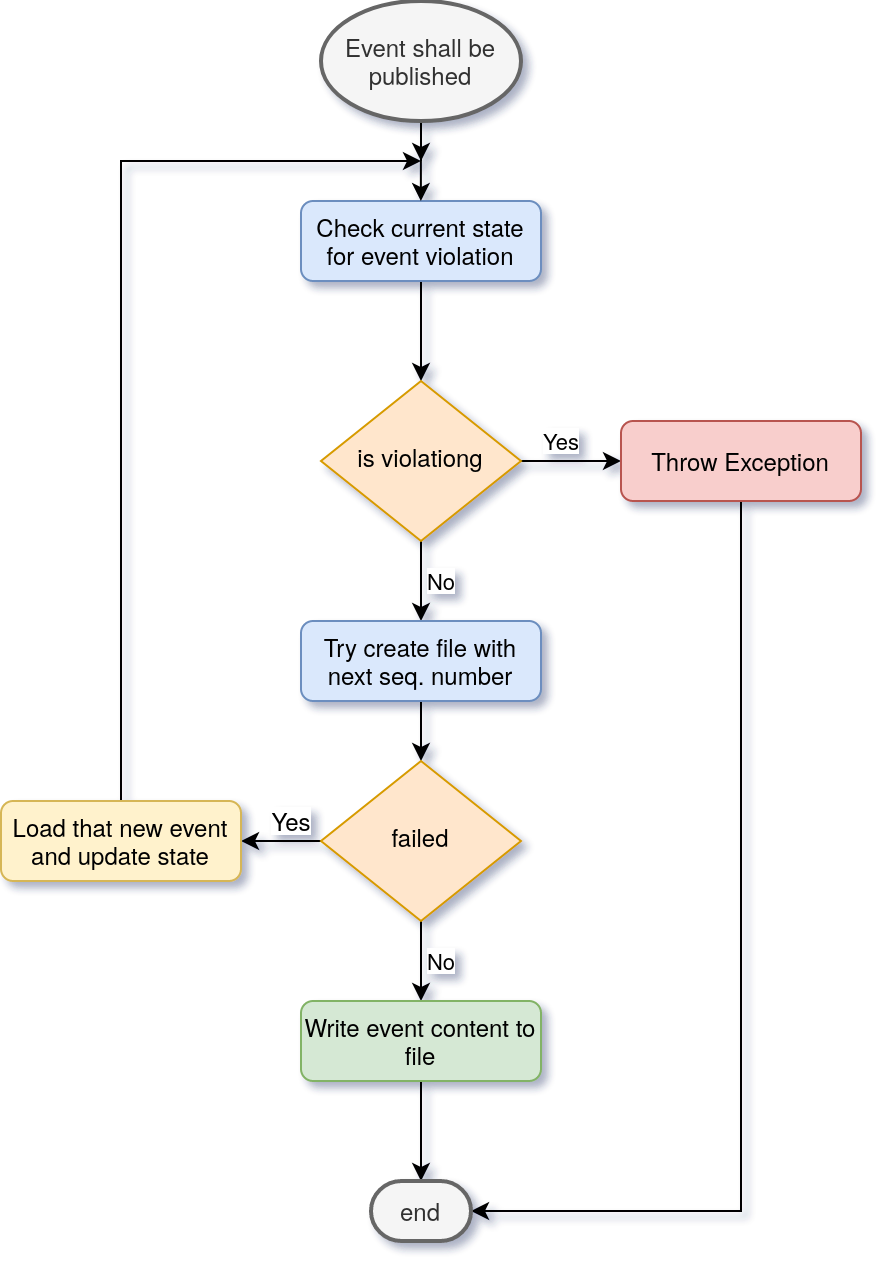
\includegraphics[width=0.4\textwidth]{event_publishing.png}
	\caption{Publishing process}
	\label{event:synchronized_publish}
\end{wrapfigure}

Every Winslow instance is responsible for keeping track of all global states and check before publishing a new event \todo{ref} whether the state would be violated by this event.
If it is not, it will try to publish it by creating a new file with the next expected sequence number.
If the file already exists, another instance did publish an event in the meantime.
This externally published event must then loaded and the global state updated before a new trial to publish its own event can be made.
Eventually, this will either lead to successfully publishing the event or failing due to state violation - for example trying to lock a project that is already locked.


This synchronization mechanism ensures that each event is only published if it is not violating any constraints, such as locking resources that are already locked.
It also allows for multiple locks and elections to happen concurrently, as long as there is no overlap.

\begin{figure}[H]
	\centering
	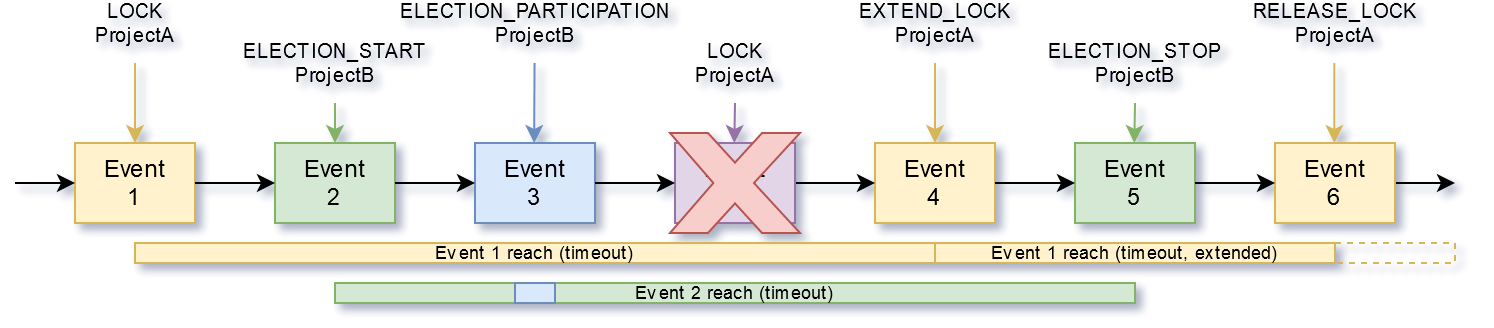
\includegraphics[width=0.9\textwidth]{events.png}
	\label{winslow:com:events}
	\caption{Sample event and lock series with lifetimes}
\end{figure}

In \autoref{winslow:com:events} a series of events, their id and commands are shown.
The coloured rectangles below shows the duration of the lifetime of events.
The crossed-out event is violating the constraint that a resource can only be locked by one instance at a time, which is the owner of the yellow lifetime in this case.
Because of this violation the even is never published to the event bus, which is demonstrate with the sequence number not skipping the number 4.

\section{Docker interface}

To interface with the Docker daemon a driver implementation is needed to pass on container creation.
Docker provides a REST API\cite{docker:api} for third party libraries as well as implementations in Go and Python.
There is no official Java API implementation.
This means, either a third party Java library must be used, the REST calls that are required have to be implemented within this project or another alternative must be found.
The Docker REST API is very expressive which is another reason to find a viable alternative.

As it turns out, the Nomad Project, which was already investigated in \autoref{nomad}, provides a library with a thin abstraction layer and lots of reasonable default values.
It also includes support to create container which use the Docker plugin by Nvidia\cite{nvidia:docker_plugin}.
This allows attaching GPUs to a container without the need of listing all libraries and device files manually\footnote{If you are interested in how tedious this could otherwise become see \url{https://github.com/hashicorp/nomad/issues/3499\#issuecomment-364214506}}.
The scheduling capabilities of Nomad are not used \todo{because: nomad focuses on scheduling multiple instances of a load balanced service, lack of control on where it is spawned, additional communication channels required -> firewall/admin/maintanance, interfer with further extenstions cloud like cloudstore and GlusteFS because a 'randomly' by nomad chosen node would require access to the storage which might not be visible to all executions nodes through the same path}.


\section{Directory Structure and Organization}

This section describe the organization of the working directory for the Winslow instances.
Because a common network share is required by Winslow for event synchronization and the projects' workspaces, this was further extended to share the configuration and project files as well.
This has the very nice side-effect, that is no real setup to do when starting a new Winslow instance, the only required input by the administrator is the path to the common network share.
Of course, special needs apply to certain directories, which will be discussed next.

For the configuration files, a principle found on Unix and Linux was applied: human readable text files.
In the case of Winslow they use YAML\todo{cite} or property\todo{.} \todo{formatting}.
This allows easy debugging in error scenarios. \todo{.}

\subsection{Winslow working directory}

A brief summary of the by all instances shared working directory:

\begin{itemize}
	\item \monospaceinline{logs}: The location for stage log files. Logs system events and console output with timestamps. File name format looks like \monospaceinline{<project-id>-<stage-number>-<stage-name>}.
	\item \monospaceinline{pipelines}: Pipeline definition file (YAML) are located here.
	\item \monospaceinline{projects}: Project definition files (YAML) are located here.
	\item \monospaceinline{resources}: The globally available input resources \todo{see ref}
	\item \monospaceinline{run/events}: The directory used to synchronized events \todo{see ref}
	\item \monospaceinline{run/nodes}: The directory used to publish node utilization \todo{see ref}
	\item \monospaceinline{settings}: The directory used to share common configurations, currently this only contains a global environment variable configuration.
	\item \monospaceinline{workspaces}: Discussed in \autoref{stage:workspace}
\end{itemize}

Because the files in \monospaceinline{run/events} and especially \monospaceinline{run/nodes} are very temporary, the NFS server locates these in shared memory (\monospaceinline{/dev/shm}) to reduce stress on IO and unnecessary wear on SSDs.

\subsection{Stage storage}
\label{stage:workspace}


Thinking about the storage organisation for the pipeline and its stages, a few expectations and concerns arise.
First of all, to redo a stage, one needs to be able to access the files that were the result of one, two or multiple stages before the current.
Sometimes a stage wants to access intermediate data produces by multiple previous stages.
Next, the input video footage needs to be accessed by multiple stages throughout the pipeline execution.
Finally, some stage results are not intermediate but final results.
\todo{examples}

The first and second concern can be solved by providing a workspace directory for each stage, that is copied from the logically previous stage.
Once the computation of a stage is completed, the workspace is considered immutable and only used to source new workspaces from.
This works fine for small intermediate results, but it does not work very well for large files - like the video footage.
Starting a new stage will take as long as the copy of multiple gigabytes on a spinning devices take (\todo{sample GB and time}), require unnecessary storage due to multiple copies and provides no benefits in an archival and version control sense, because the video footage is not altered.
So there needs to be another storage pool for input data, that is globally accessible and never changed: the global input storage pool.
Providing one further storage pool for final results (global output pool), concern number three and four are also solved.

Because the very first stage has no workspace to source its files from, on creation of the pipeline a workspace directory for the \enquote{zeroths} stage is created.
The user can then provide the very first stage with a predefined and non-empty workspace if necessary.

Because in the implementation of this project NFS was used, this also solves one further problem that was experienced in the prototyping phase: copying files on NFS (and many other network filesystems like Samba) is a client operation.
This means, the client reads the input file and writes to the output file.
Because the common network used (gigabit in this case) is slower than spinning disk sequential read/writes (network: 112 Megabytes/s in theory, divided by two because read+write on the same connection: 56 Megabytes/s, spinning enterprise disk: about 170 Megabytes/s \todo{test on johnny5}), this operation does not only take unnecessary long but also renders the network connection close to unusable for any other participant in the network that needs to use parts of the same physical route.

To ensure that the global input and the previous intermediate results are not altered, the Docker daemon is instructed to mounted them as read-only filesystems.
This makes it impossible\footnote{When there is no bug in the implementation of mount or Docker} for the stage to accidently delete or alter the wrong files\footnote{Like in this scenario, where an unexpected space in a script caued people to loose their home directory: \todo{steam rm -rf incident}}.


\begin{figure}[H]
	\centering
	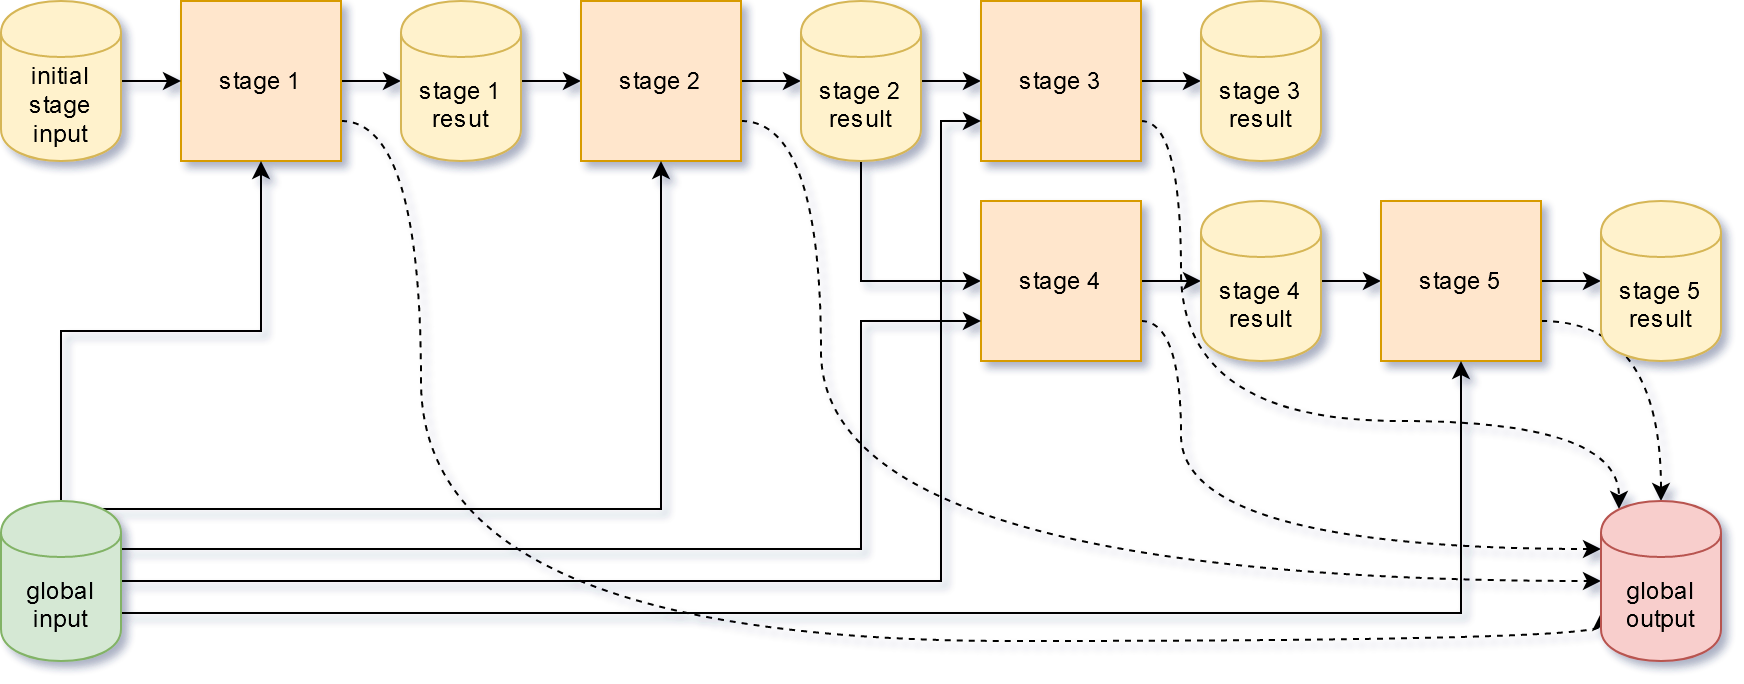
\includegraphics[width=0.9\textwidth]{stage-storage.png}
\end{figure}

In summary, the storage pool solution looks like this:

\todo{check paths}
\begin{itemize}
	\item \monospaceinline{/input} is mounted read-only from \\ \monospaceinline{nfs-server:/winslow/workspaces/<pipeline-id>/input}
	\item \monospaceinline{/output} is mounted with write permissions from \\ \monospaceinline{nfs-server:/winslow/workspaces/<pipeline-id>/output}
	\item \monospaceinline{/workspace} is mounted with write permissions from \\ \monospaceinline{nfs-server:/winslow/workspaces/<pipeline-id>/<stage-id>} \\
	and was created by the copying the workspace directory of the logically previous stage
\end{itemize}

\todo{define logically previous stage -> previous stage on linear execution and ... when jumping around}



initial input

stage execution does not need to depend on the result of the exact previous



\section{Job Scheduling / Election System}
\label{design:election}

\subsection{Affinity and Aversion}
\label{election:affinity_and_aversion} \todo{.}

\todo{affinity}
\todo{aversion}

Utilizing Event Bus for timely limited elections and to ensure that there are no concurrent election for a single project.

\todo{what about concurrent elections on multiple projects}

\todo{regarding locking: check for updatable, try to lock, check for updatable again, update, unlock}

\todo{on unlock: check updatable}



\todo{scheduling / job assignment/pull strategy}

\todo{graph displaying over time lock and election}


\section{CPU RAM Network IO Monitoring}

\section{User Interface}

\todo{REST request, read only: no lock; for changes: POST -> LOCK -> update -> RELEASE, on RELEASE Winslow gets notified and checks whether the new configuration leads to a new stage execution}

\subsection{Spring Boot}
\label{design:springboot}
\todo{spring boot}

\begin{comment}
\section{File system}

\todo{docker can auto mount nfs to container}

\subsection{Every node has a connection to every other node}

\subsection{Centralized broker}

\subsection{Tree hierarchy}

\subsection{outcome}




\section{Communication and Node Management}

The system that shall be developed, is supposed to spread jobs onto execution nodes as available.
There are two main approaches in nod management and job assignment.



\subsection{Centralized Management, Remote Execution}

In the central management approach, there is always exactly one leader at any given moment in time.
It is the responsibility of this leader to decide what to execute and where to execute it.

\subsection{Decentralized Management, Local Execution}

\subsection{Combinations worth noting}

stupid:
 - centralized management, local execution
 - decentralized management, remote execution
 
combination, decentralized + some remote slaves

\subsection{Architecture}

event based

common file system for communication because minimum requirements

stick to unix principles(list): simple, human readable intermediate format

voting/election by capabilities and 'will' of a node to run a stage

\todo{providing live hw utilization}

\todo{the whole properties thingy}

\subsection{Failure handling}
\todo{handling failed stages}

\todo{handling failed nodes}

\section{Communication/Event architecture?}

\section{Targeting capabilities}

\subsection{General thoughts}

\section{Planned}

\section{Implementation details}

\section{Synchronization, Locking, publishing events}

\section{REST for UI}



\subsection{Atomicy of (Unix) Filesystems}

\subsection{Atomicy and behavior of NFS in particular}

\subsection{Using as lock backend}

\subsection{Using as election backend}
\end{comment}




\section{Agile development}

\todo{.depends, maybe to shallow and not worth noting, dont forget to then ref to \autoref{fundamental:agile}}


\section{Continuous Deployment}

Ironically, although mentioned as unusable in \autoref{.}\todo{.} for the use case Winslow wants to fulfil, it will use GitLab CI for continuous \todo{delivery} of runnable Docker Images.
Every code change in the Git repository will trigger a new build pipeline, that builds and tests Winslow, packages all dependencies \todo{nomad} into a Docker image and pushes it to our in house private Docker Registry \todo{.}.
The \todo{execution nodes} will pull the latest image whenever they restart or are triggered to restart.
\todo.